\section{Additional Figures}
\label{app:figures}

This appendix collects supplementary figures. The headline figures
(whale density sweep, $\psi_W$ vs $\psi_t$ influence functions, and
the Hillstrom Hill plot) appear inline in
\S\ref{sec:experiments}. All are reproducible from the scripts
in \texttt{benchmarks/} of the code release.

\begin{figure}[!t]
  \centering
  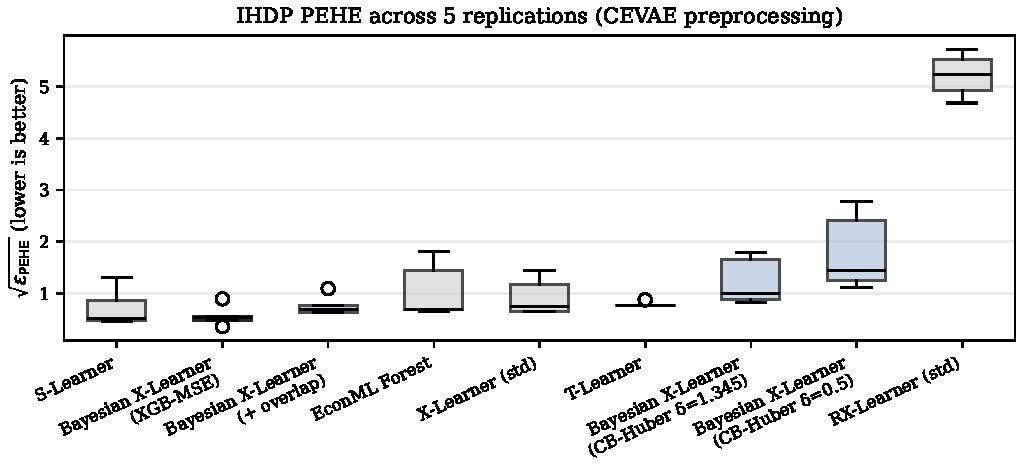
\includegraphics[width=\linewidth]{figures/fig2_ihdp_pehe.pdf}
  \caption{$\PEHE$ distribution across 5 IHDP replications. Each
    box spans the inter-quartile range; whiskers extend to
    min/max. The Bayesian X-Learner with XGB-MSE nuisance (dark
    blue) wins; the CB-Huber variants (light blue) are included to
    make the clean-data efficiency cost visible and are not
    competitive entries.}
  \label{fig:ihdp_pehe}
\end{figure}

\begin{figure}[!t]
  \centering
  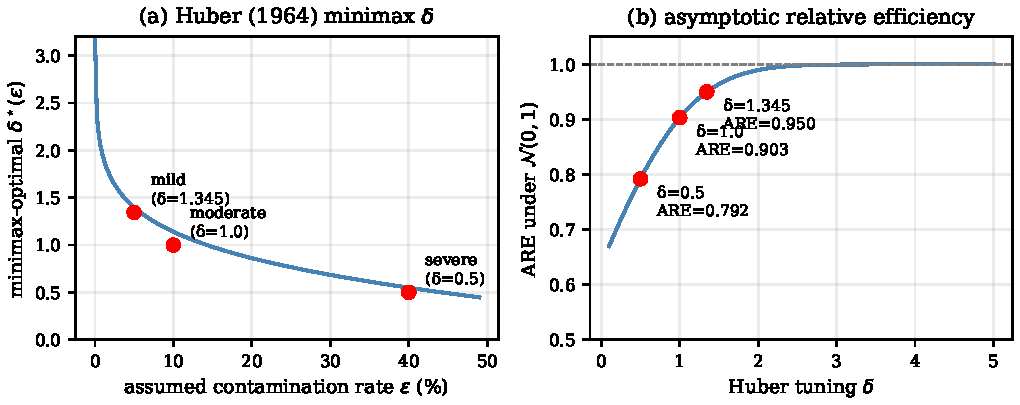
\includegraphics[width=\linewidth]{figures/fig3_huber_curves.pdf}
  \caption{Huber's (1964) minimax-$\delta$ and asymptotic relative
    efficiency. \textbf{(a)} Solution of
    \eqref{eq:huber_minimax} for $\delta^\star(\epsilon)$, with
    the three Huber-nuisance presets marked.
    \textbf{(b)} ARE$(\delta)$ under the Gaussian centre. Numerical
    values match~\citet{huber2009robust} Table 4.1: ARE $= 0.950$
    at $\delta = 1.345$ (mild) and $0.792$ at $\delta = 0.5$
    (severe). The observed IHDP PEHE penalty is much larger than
    these ARE values alone predict; see
    \S\ref{sec:experiments:efficiency}.}
  \label{fig:huber_curves}
\end{figure}

\begin{figure}[!t]
  \centering
  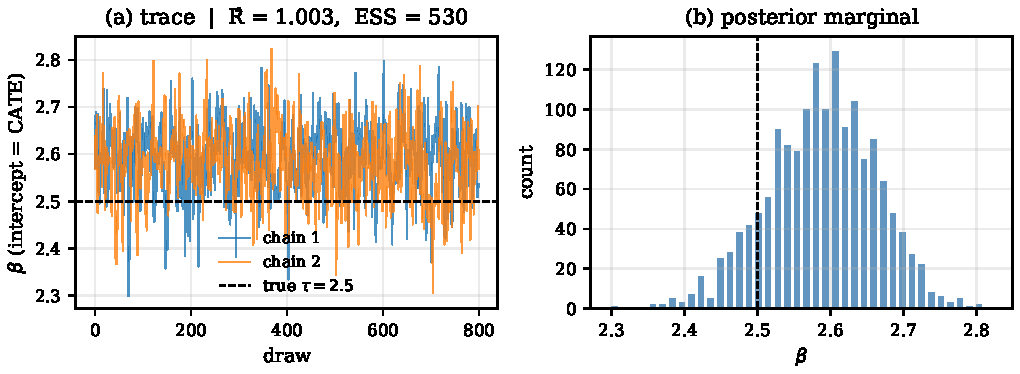
\includegraphics[width=\linewidth]{figures/fig4_posterior_traces.pdf}
  \caption{Representative MCMC trace and posterior marginal from a
    clean-data fit ($N = 500$, intercept basis, true $\tau = 2.5$).
    \textbf{(a)} Two chains overlap cleanly around the true value;
    $\hat{R}$ and effective sample size are reported in the panel
    title. \textbf{(b)} Pooled posterior marginal. This pattern
    --- $\hat{R} < 1.05$, $\mathrm{ESS} > 200$, 100\% of runs --- is
    typical across every benchmark reported in
    \S\ref{sec:experiments} and
    Appendix~\ref{app:convergence}.}
  \label{fig:traces}
\end{figure}

\begin{figure}[!t]
  \centering
  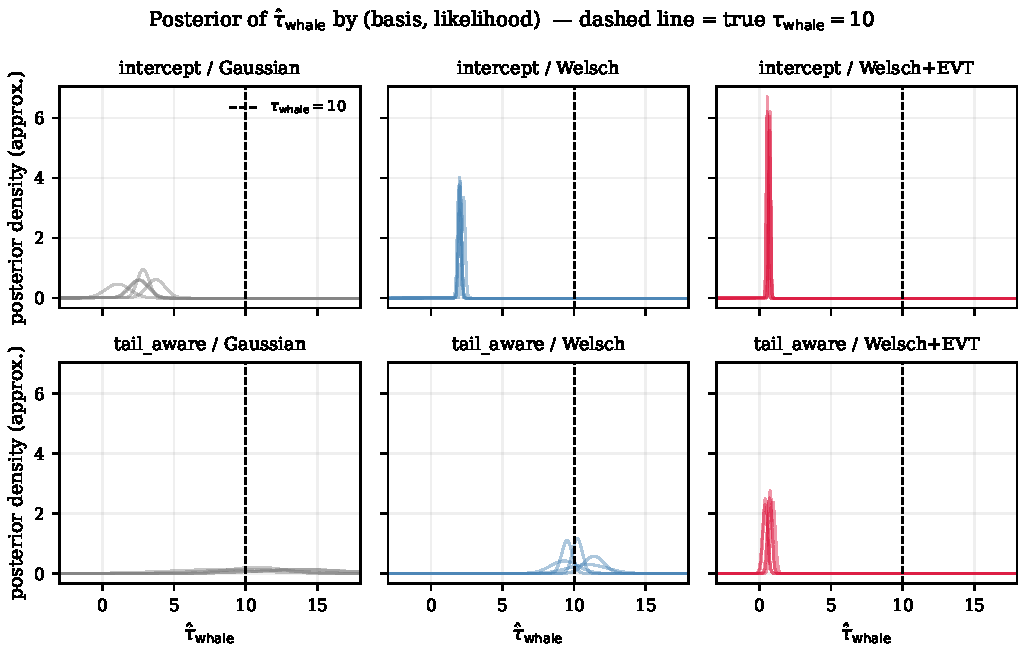
\includegraphics[width=\linewidth]{figures/fig5_tail_posteriors.pdf}
  \caption{Approximate posterior densities of $\hat\tau_{\text{whale}}$
    for each (basis, likelihood) combination in
    Table~\ref{tab:tail_signal}. The tail-aware + Welsch cell (top
    middle column, bottom row) places posterior mass around the
    true $\tau_{\text{whale}} = 10$; the
    \texttt{normalize\_extremes} cells (right column) collapse the
    posterior to near zero, visibly demonstrating that the
    data-layer rescaling removes tail signal. Densities are
    Gaussian approximations centred at the posterior mean with
    $\sigma$ from the 95\% CI width, one curve per seed.}
  \label{fig:tail_posteriors}
\end{figure}
